\subsection{Adaptive Walking Motion}
When the passive walker walks down a slope, for every step, there is energy input from the potential energy,
and there is also energy loss because of heel strike. 
There must be an equilibrium condition when the energy lost is equal to the energy input. 
If natural looking motion is energy efficient, such passive walking motion can be expected to be natural looking. 
Because there is no extra control energy input, such motion is the most energy efficient.

\begin{figure}[H]
\centering
\includegraphics[width=5inch]{\figurepath/passive_walking.eps}
\caption{Stable passive walking gait}
\label{fig:passive_walk}
\end{figure}
Figure \ref{fig:passive_walk} shows the gait of the passive walker. 
After coupling the neural oscillator, the basic pattern is not changed  as shown in \figurename ~\ref{fig:stable_active_walk}.

\begin{figure}[H]
\centering
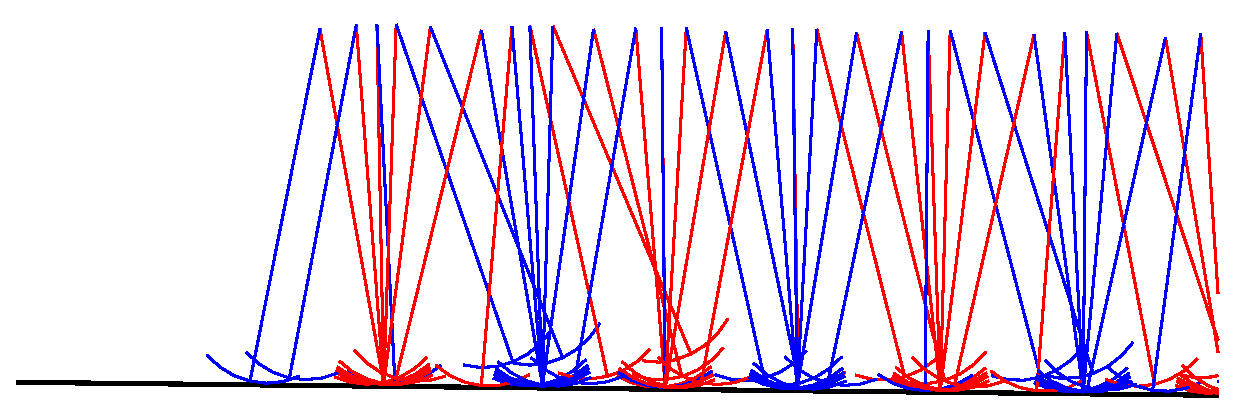
\includegraphics[width=5inch]{\figurepath/actuated_walk_downslop.eps}
\caption{Walk down the same slop when actuated}
\label{fig:stable_active_walk}
\end{figure}

However the stability is fragile.  
The passive walker can't walk on plane. 
The step size will decrease after each step, and finally it will stop or fall over as illustrated in \figurename ~\ref{fig:pass_waling_on_plane}.
\begin{figure}[!h]
\centering
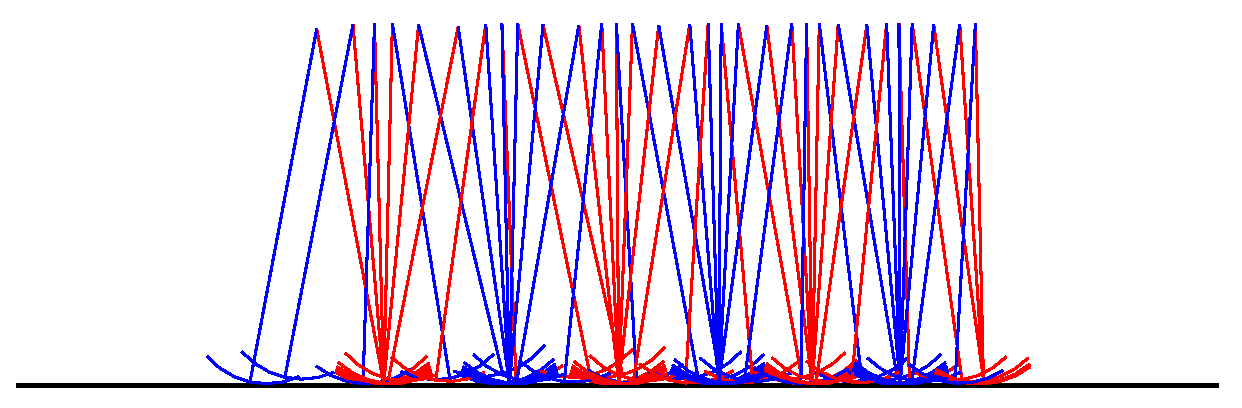
\includegraphics[width=5in]{\figurepath/passive_walk_on_plane.eps}
\caption{Passive walking gait can't be maintained on plane}
\label{fig:pass_waling_on_plane}
\end{figure}

After coupled with the neural oscillator, this walking machine can walk on plane, and exhibits gait similar to the passive dynamic walker. 
\figurename ~\ref{fig:walk_plane} shows the gait. 
From the state plot \figurename ~\ref{fig:walk_plane_state}, and phase plot \figure ~\ref{fig:walk_plane_phase}, we can see that the gait converged to a stable limit circle.

\begin{figure}[!h]
\centering
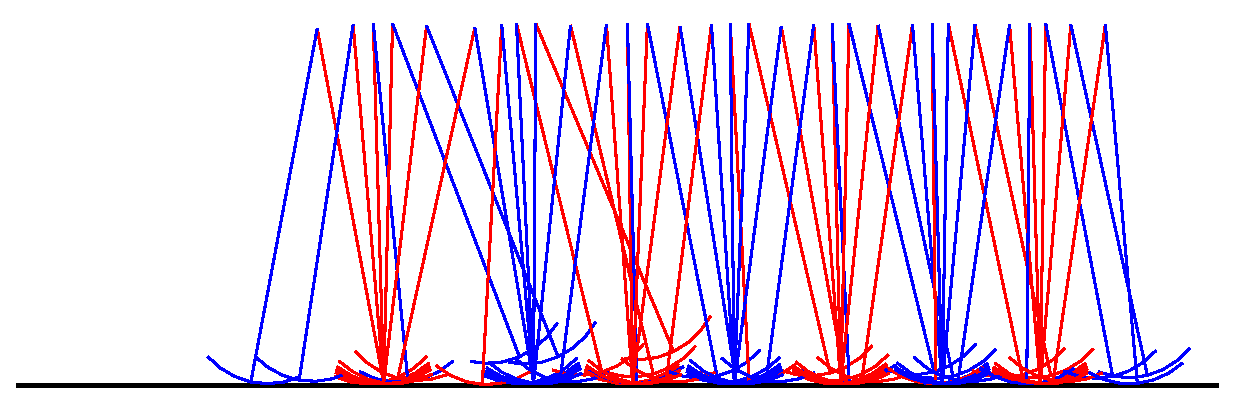
\includegraphics[width=5in]{\figurepath/walker_on_plane.eps}
\caption{Walking on plane under neural control}
\label{fig:walk_plane}
\end{figure}


\begin{figure}[!h]
\centerline{
\subfigure[State Plot]{
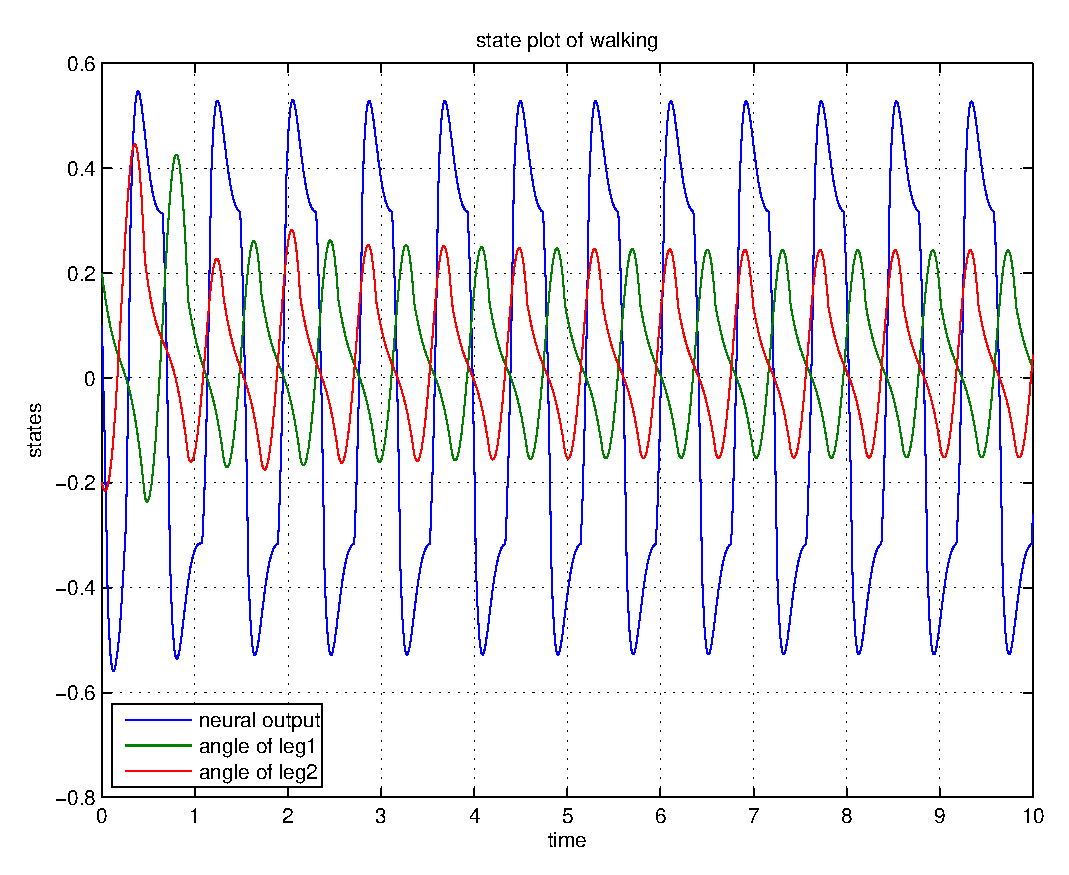
\includegraphics[width=3in]{\figurepath/walking_on_plane_time_state}
%\label{fig:walk_plane_state}
}
\hfill
\subfigure[Phase Plot]{
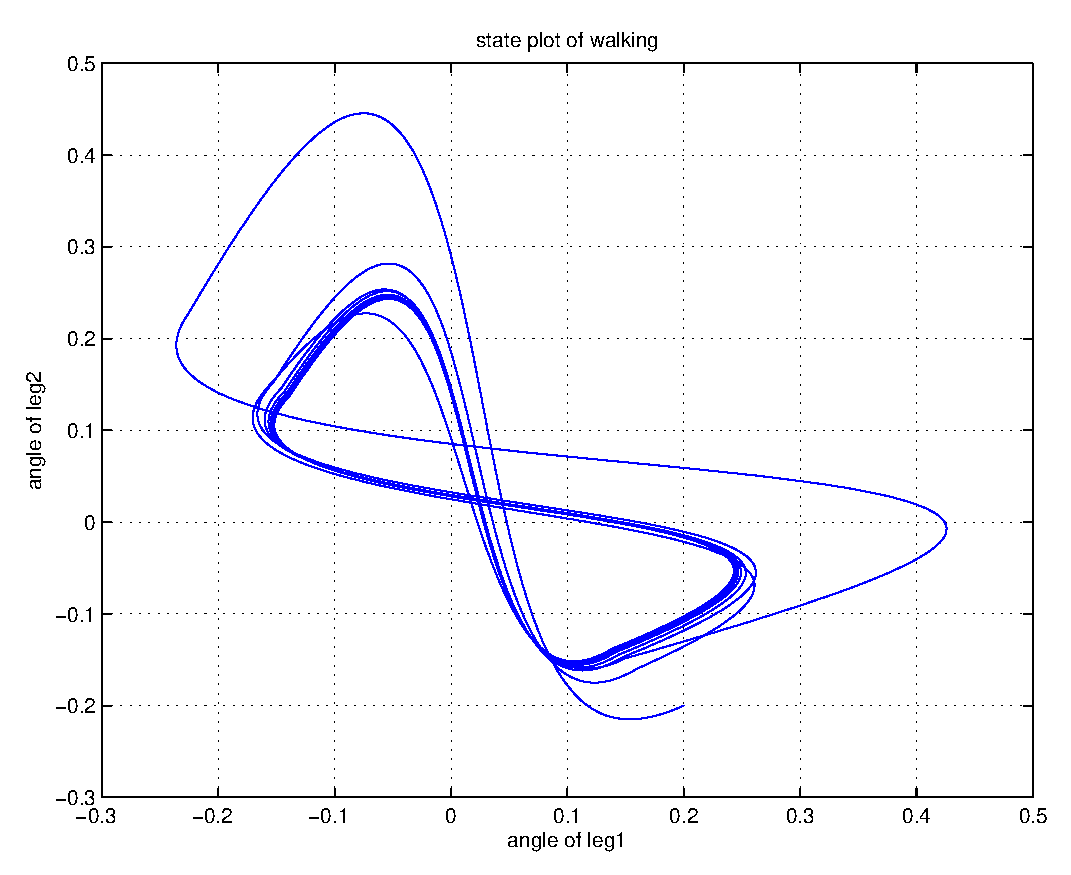
\includegraphics[width=3in]{\figurepath/walking_on_plane_phase.eps}
%\label{fig:walk_plane_phase}
}
}
\caption{
Walking on a plane converges to a stable limited circle
}
\label{fig:walk_on_plane}
\end{figure}
To verify the structural stability, we introduce a variety of perturbations to the passive walker. 
These perturbations include different initial condition, different slopes, different leg mass and different leg length.
\begin{description}
\item [Different Initial Condition]
The original passive walker is not very stable. 
A slight change in initial condition will result in walking failure. 
While after coupled with neural oscillator, the basin of attraction has been enlarged. 
A different initial condition can still lead to a stable gait, as show in Figure \ref{fig:diff_init}. 
Natural looking gait is maintained.
\begin{figure}[h]
\centering
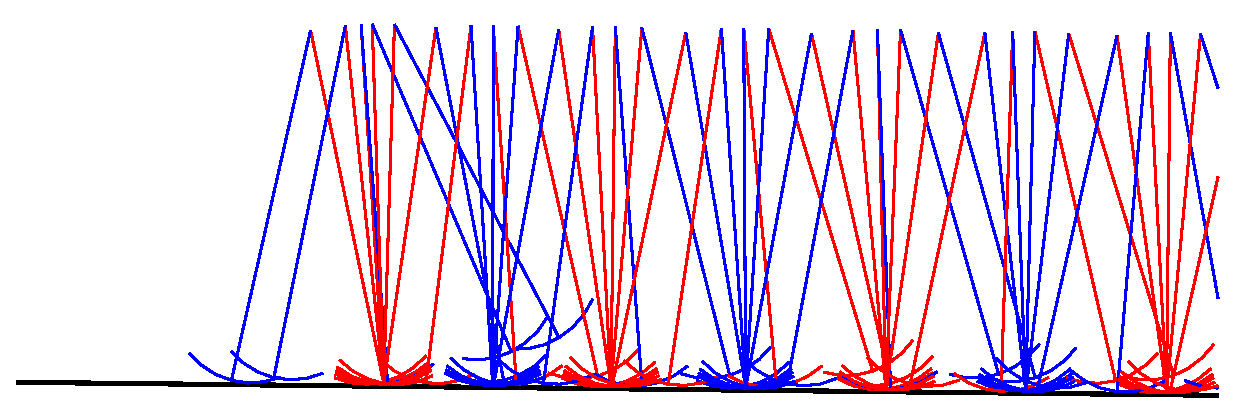
\includegraphics[width=5inch]{\figurepath/walk_down_with_differnt_init_cond_suceed.eps}
\caption
{
Walking with different Initial condition
}
\label{fig:diff_init}
\end{figure}
 

\item[Walking On Different Slopes]
Another parameter we change is angle of the walking slope. 
When we increase the down slope, stable walking motion can still be maintained, as shown in figure \ref{fig:diff_slop}.
An important discovery is that although the walkers can walk on various down slopes, it can not walk up slope,no matter how control parameters are changed.
It can’t walk up slope and will fall backward after several steps. 
We suggest that this is because the proper limit circle does not exist in the dynamic system when walking up slope.
This finding may help us to understand the upper body effect in walking.

\begin{figure}[here]
\centering
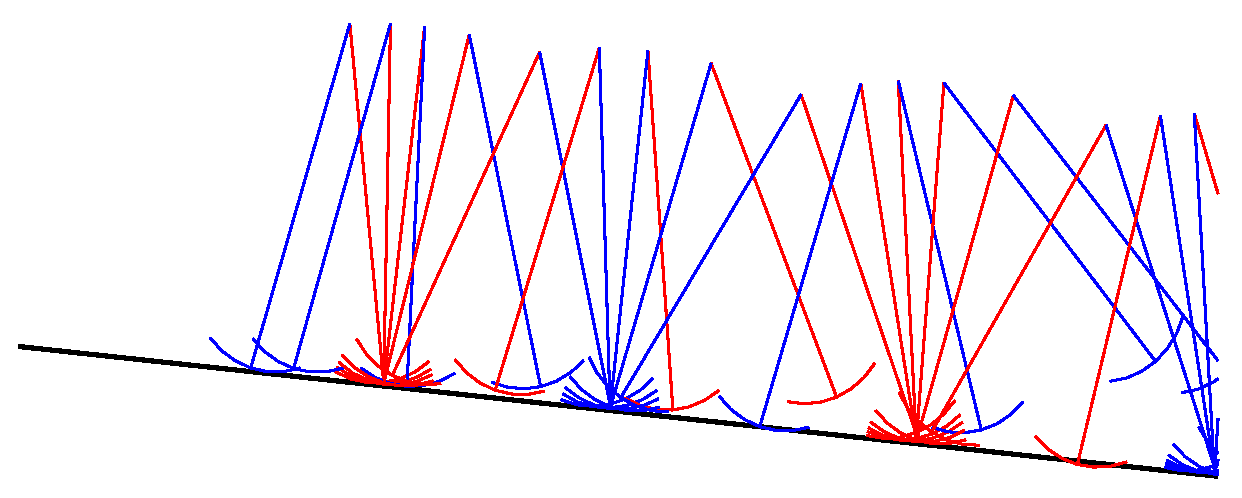
\includegraphics[width=\textwidth]{\figurepath/big_slop_actuated_suceed.eps}
\caption
{
Walking with different slope angle
}
\label{fig:diff_slop}
\end{figure}

\item[Leg Mass Variation]
We add mass on one leg to 50\% and find the stability of the gait is still maintained. 
The step length and swing period of the two legs are different, this gait is similar to that with a crippled leg, see figure\ref{fig:leg mass}.

\begin{figure}[here]
\centering
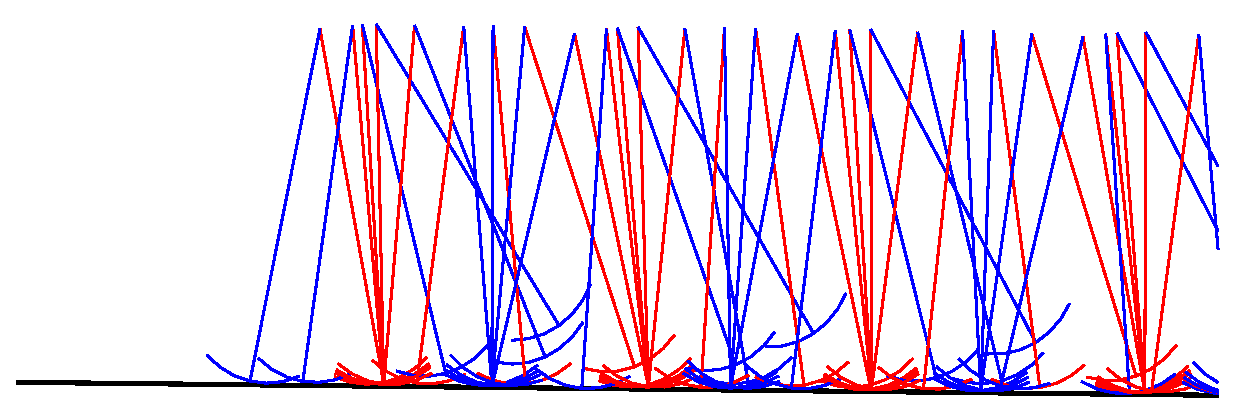
\includegraphics[width=5in]{\figurepath/walk_mass_changed.eps}
\label{fig:walk_mass_changed}
\caption
{
Walking with legs of different mass
}
\label{fig:leg mass}
\end{figure}

\item[Leg Length Variation]
The last parameter we change is the leg length. 
We change the leg length to 1/8 shorter. 
And we find the stability of the gait is maintained, see \figurename ~\ref{fig:walk_leg_changed}

\begin{figure}[h]
\centering
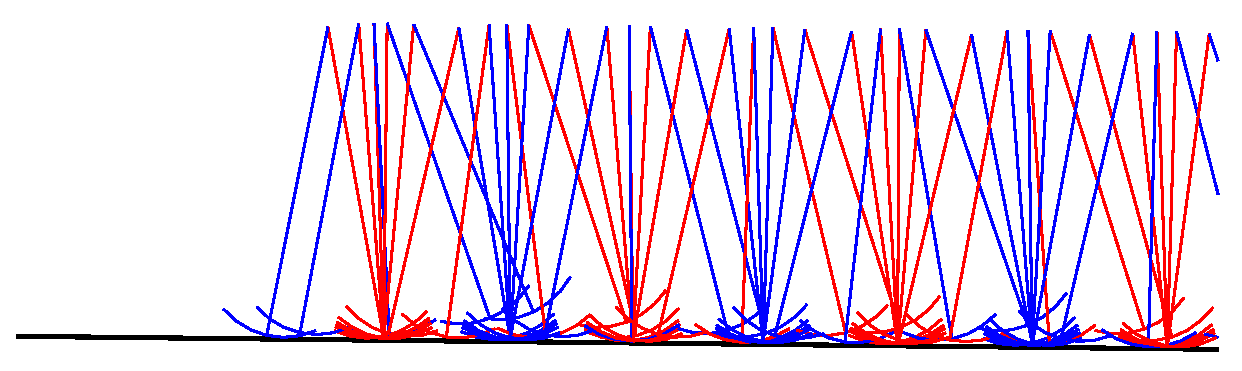
\includegraphics[width=5in]{\figurepath/walk_leg_changed_success.eps}
\caption
{
Walking with shorter Legs
}
\label{fig:walk_leg_changed}
\end{figure}
\end{description}

The method of nonlinear entrainment did boost the structure stability and can result in stable motion under different environment change.
By making walking a structure stable autonomous system, natural looking and adaptive motion are generated, without planning the motion curve.
